\documentclass[12pt]{beamer}

\usepackage{color}
\usepackage[T2A]{fontenc}

\usepackage[absolute,overlay]{textpos}
\usepackage{setspace}
\usepackage[export]{adjustbox}
\usepackage{wrapfig}
\usepackage{csquotes}

\defbeamertemplate{footline}{centered page number}
{%
  \hspace*{\fill}%
  \usebeamercolor[fg]{page number in head/foot}%
  \usebeamerfont{page number in head/foot}%
  \insertpagenumber\,/\,\insertpresentationendpage%
  \hspace*{\fill}\vskip2pt%
}
\setbeamertemplate{footline}[centered page number]
%\mode<presentation>{
%\usetheme{Rochester}
%}
\newcommand{\backupbegin}{
   \newcounter{framenumberappendix}
   \setcounter{framenumberappendix}{\value{framenumber}}
}
\newcommand{\backupend}{
   \addtocounter{framenumberappendix}{-\value{framenumber}}
   \addtocounter{framenumber}{\value{framenumberappendix}} 
}
\mode<presentation>{
  \usetheme{AnnArbor}
}
\makeatletter
\setbeamertemplate{footline}
{
  \leavevmode%
  \hbox{%
  \begin{beamercolorbox}[wd=.333333\paperwidth,ht=2.25ex,dp=1ex,center]{author in head/foot}%
    \usebeamerfont{author in head/foot}\insertshortauthor%~~\beamer@ifempty{\insertshortinstitute}{}{(\insertshortinstitute)}
  \end{beamercolorbox}%
  \begin{beamercolorbox}[wd=.333333\paperwidth,ht=2.25ex,dp=1ex,center]{title in head/foot}%
    \usebeamerfont{title in head/foot}\insertshorttitle
  \end{beamercolorbox}%
  \begin{beamercolorbox}[wd=.333333\paperwidth,ht=2.25ex,dp=1ex,right]{date in head/foot}%
    \usebeamerfont{date in head/foot}\insertshortdate{}\hspace*{2em}
    \insertframenumber{} / \inserttotalframenumber\hspace*{2ex} 
  \end{beamercolorbox}}%
  \vskip0pt%
}
\makeatother

\setbeamertemplate{navigation symbols}{}

\setbeamercolor{frametitle}{fg=black,bg=white}
\setbeamercolor{title}{fg=black,bg=yellow!85!orange}

\beamersetuncovermixins{\opaqueness<1>{25}}{\opaqueness<2->{15}}


\begin{document}

\title{Probabilistic machine learning}
\author{Victor Kocheganov}
\date{\today} 

%\begin{frame}
%\titlepage
%\end{frame}

%\begin{frame}\frametitle{Agenda}\tableofcontents
%\end{frame} 

\section{Bayesian machine learning}


\begin{frame}{Bayesian inference main idea}
Given prior parameter distribution 
$$
P(\theta)
$$
Find its posterior distribution, given training data
$$
P(\theta|D)
$$
and use it for test data
$$
P(D_{\text{test}}|D) = \int P(D_{\text{test}}|\theta,D)\times P(\theta|D) d\theta
$$
\end{frame}


\begin{frame}{Medical diagnosis problem}
\begin{figure}
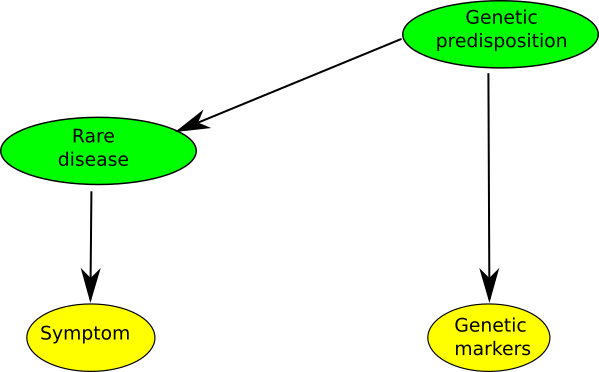
\includegraphics[scale=0.3]{medical.png} 
\end{figure}
Model = Graph (dependencies) + Conditional Probs

\begin{multline*}
P\left(R\_D = F | S = T, G\_M=F\right)=\frac{P\left(S = T | R\_D = F\right)}{P\left(S=T |G\_M=F\right)} \times \\ 
\times{\color{red}\sum_{\alpha\colon G\_P=\alpha} }P\left(R\_D=F|G\_P=\alpha\right)\times P\left(G\_P=\alpha|G\_M=F\right)
\end{multline*}
\end{frame}

\begin{frame}{Markov Random Fields}
\begin{figure}
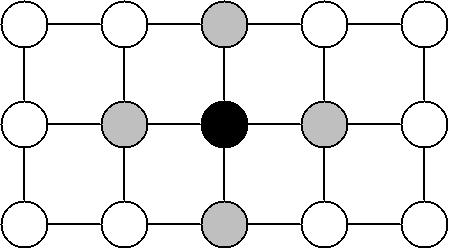
\includegraphics[scale=0.2]{MRF.jpg} 
\end{figure}
\begin{figure}
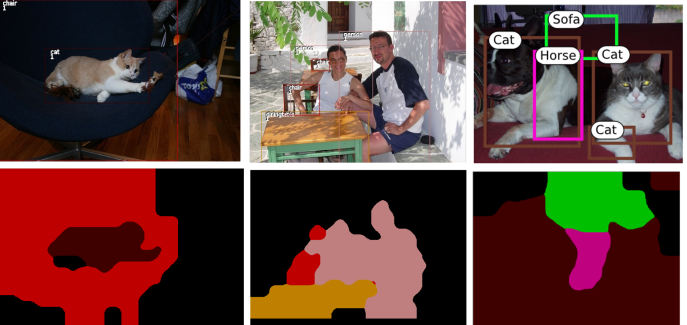
\includegraphics[scale=0.7]{MRF_example.png} 
\end{figure}
\end{frame}

\begin{frame}{Flexibility of ML models}
There are two ways of achieving flexibility:
\begin{enumerate}
    \item Large number of parameters compared with dataset (e.g. neural network can have 300 millions); Fit the parameters
    \item Non-parametric model. Complexity grows with the amount of trainig data. Fit the data.
\end{enumerate}
\end{frame}

\begin{frame}{Gaussian process model}
\begin{block}{Definition}
$\left\{F(x)\right\}$, $x\in R$, is called Gaussian Process, if for any sequence $x_1<x_2<\ldots<x_m$ vector $\left(F(x_1),F(x_2),\ldots,F(x_m)\right)$ has multivariate normal distribution.
\end{block}
%$\left(f(x)\right)$, $x\in R$ --- sample from $\left\{F(x)\right\}$.
$\left\{F(x)\right\}$ is specified by $(m(x);K(x_1,x_2))$ --- mean and covariance functions.

{\color{blue}Priors}:
\begin{align*}
m(x)&=m,\\
K(x_1,x_2)&=\theta_0 \exp{\left(-\frac{1}{2}(x_1-x_2)^2/\theta^2\right)}.
\end{align*}

\end{frame}

\begin{frame}{Bayesian optimization}
\begin{figure}
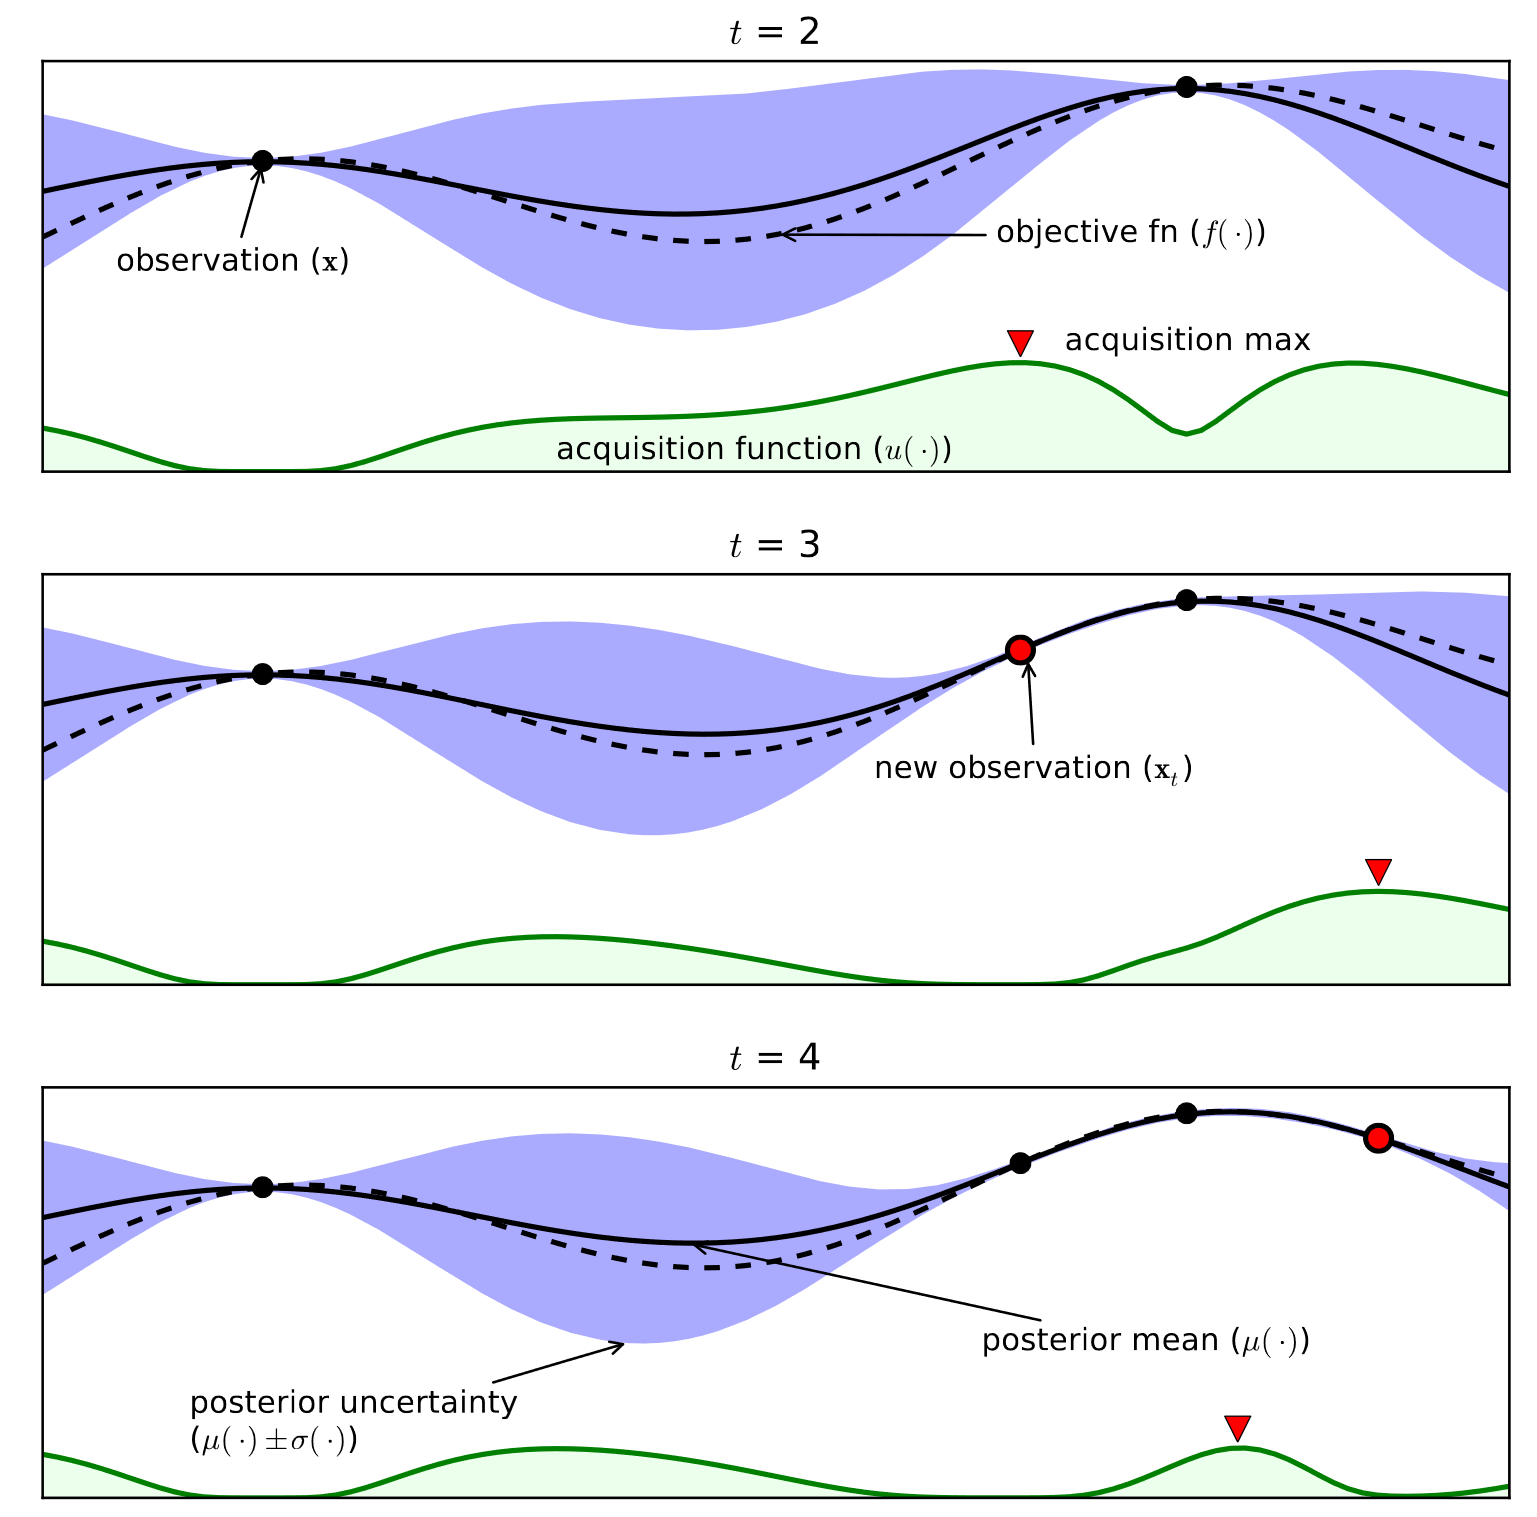
\includegraphics[scale=0.35]{Bayes_optimization.png} 
\end{figure}
\end{frame}

\begin{frame}{Bayesian optimization}
Given training data calculate posterior Gaussian Process with 
$$
\mu(x,\{x_n,y_n\},\theta), \quad \sigma(x,\{x_n,y_n\},\theta).
$$

Given posterior distribution, calculate next point:
$$
x_{\text{next}}=arg\,max_{x}a(x)
$$
where $a(x)$ is an acquisition function, e.g.
$$
a_{\text{PI}}(x;\{x_n,y_n\}, \theta)=\Phi(\gamma(x)),\quad \gamma(x)=\frac{f(x)_{\text{best}} - \mu(x,\{x_n,y_n\},\theta)}{\sigma(x,\{x_n,y_n\},\theta)}
$$
\end{frame}


\begin{frame}{Bayesian optimization}
Branin-Hoo function:
$$
f(x_1,x_2) = a(x_2-bx_1^2+cx_1 - r)^2 +s (1-t)cos(x_1)+s,
$$
where $x_1\in [-5;10]$ and $x_2\in [0;15]$.
\end{frame}

\end{document}
